\documentclass[conference]{IEEEtran}
\IEEEoverridecommandlockouts
% The preceding line is only needed to identify funding in the first footnote. If that is unneeded, please comment it out.
\usepackage{cite}
\usepackage{amsmath,amssymb,amsfonts}
\usepackage{algorithmic}
\usepackage{graphicx}
\usepackage{textcomp}
\usepackage{xcolor}
\usepackage{tabularx}

\usepackage{fancyhdr}
\pagestyle{fancy}
\lhead{Michigan Robotic Submarine}
\rhead{\thepage}

\def\BibTeX{{\rm B\kern-.05em{\sc i\kern-.025em b}\kern-.08em
    T\kern-.1667em\lower.7ex\hbox{E}\kern-.125emX}}
    
\begin{document}

\title{Michigan Robotic Submarine: Strategy, Design, and Implementation of Wettstein}
\author{
Nolan Kuza, Muhammad Bahru Sholahuddin, Diego Montemayor, Kathryn Wakevainen \\
Kobi Wettstein, Adarsh Ponaka, Elaina Mann, Melissa Peters, Arnav Mummineni, Jennifer Chin, \\ Alexander Bowler, Tong Sing Wu, Shrey Sahgal, Emi Yuki, Shubh Agrawal, Andrew Huston \\
% TODO add rest of names
}

\maketitle
\pagestyle{fancy}
\lhead{Michigan Robotic Submarine}
\rhead{\thepage}

\begin{abstract}
Michigan Robotic Submarine is an undergraduate student project team at the University of Michigan in its fourth year participating in the RoboSub competition. We developed our autonomous underwater vehicle (AUV), Wettstein, shown in Fig. 1, to advance our capabilities to new tasks while also addressing the limitations of our previous design. To improve the robustness and maintainability of our system, we added thruster guards and designed two new custom PCBs. We have also developed a strong foundation for flexible software, which we leveraged to create software best-suited for this year's task, including a streamlined pipeline for classical computer vision algorithms and a refined task planning framework. Furthermore, we designed two mechanisms to enable new proprioceptive capabilities.

% Over the past year, our software team has developed a control interface for our AUV that enables the rapid creation of modular autonomous strategies, which are strung together to complete tasks. In tandem with these autonomous strategies, we run closed-loop controllers and machine learning-based computer vision strategies to stabilize on three axes of motion. With a more maneuverable, robust AUV, in addition to a new, higher-compute on-board computer, our software team was able to program a competition strategy that will allow us to surpass any of our previous competition runs.

%We re-worked our electrical system design to have considerably higher compute power, increasing the speed and accuracy of our deep learning-based object detection system. We also created a robust testing infrastructure that allows us to quickly and efficiently tune control parameters, diagnose software bugs, and analyze the efficacy of our AUV while in the water.
\end{abstract}

\section{Competition Strategy} \label{sec:comp_strat}
This year we focused on expanding to new tasks, and adapting to the modified tasks, such as the change in the buoy shape. Our recent enhancements to our system demonstrate its strong foundation and its ability to continuously expand to tackle this year’s and future years’ RoboSub challenges. Some areas that we identified as strengths included our machine learning pipeline, which we were able to quickly train and utilize at the 2023 competition along with a robust task planner to map out the failure cases and fallback states for each task. In turn, we chose to focus on developing our classical computer vision pipeline and designing additional mechanisms. We also designed and manufactured a thinner lid to the hull of Wettstein to reduce the weight which will earn us more bonus points.

% //After our second in-person RoboSub competition in 2023, we found that the new system we developed was much more flexible within the competition environment. 

\subsection{Target Tasks} \label{ssec:target_goals}
Our target tasks for the 2024 RoboSub competition are the coin flip, gate, buoy, and bin tasks.
\begin{enumerate}
\item \textit{Rough Seas---Coin Flip:}
To complete the coin flip task, our design requires the robot to be sensing its environment before starting the run so that it can record the angle that the gate is present at. This provides a reliable method for identifying the initial angle needed to turn to face the gate, regardless of the result of the coin flip. 
\item \textit{Enter the Pacific---Gate:}
To pass through the gate, we use a machine learning model to detect the image on the gate and center on it. We decided to always choose the same image to center on, as this allows us to focus on optimizing the model’s performance for that specific image. Additionally, this makes it so that we can complete the buoy and the bin tasks in the same way every run to maximize points (namely, the direction to circumnavigate the buoy and the color to target on the bin), enabling more consistency throughout our runs.
\begin{figure}
    \centerline{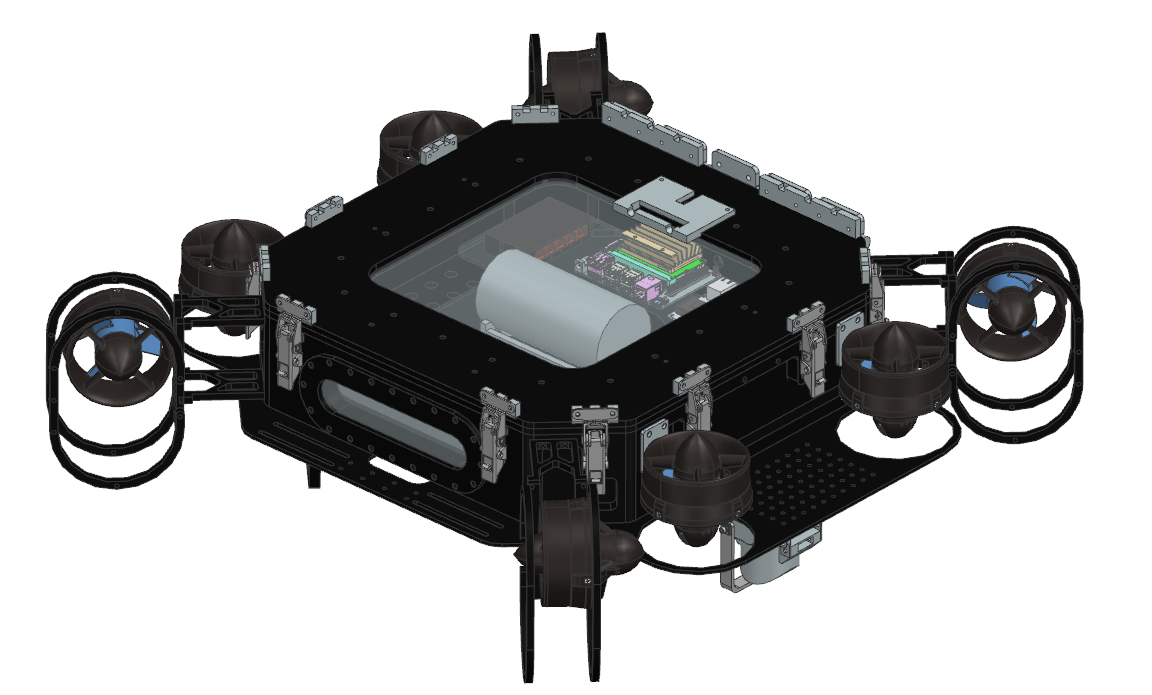
\includegraphics[scale=0.17]{images/fullSub2024.png}}
    \caption{CAD of our 2023-2024 AUV, Wettstein.}
    \label{fig:sub4}
\end{figure}
\item \textit{Path:}
In order to reach the buoy and bins tasks, we intend to use the path-marker, which requires an additional camera on the bottom of the submarine
%(see section \ref{sssec:path_marker})
. Since we use classical computer vision algorithms for our relatively low-resolution bottom camera, this sub-system draws a reasonably low amount of computing power. Should this system fail, we can use a hard-coded “fallback” orientation, making the system sufficiently reliable to be worth its associated complexity.
\item \textit{Hydrothermal Vent---Buoy:}
We also aim to achieve maximum points on the buoy task by identifying, approaching, and properly circumnavigating the buoy. To identify the buoy, we utilized the large horizontal field of view (110°) of our front-facing stereo camera along with a computer vision algorithm to detect the buoy based on its shape and color. We decided to use a classical computer vision algorithm rather than machine learning for this task since classical algorithms excel at detecting simple colors and shapes, and do not require the extensive data and training that machine learning does. To circumnavigate, we stop approaching the buoy once it has a certain radius within the camera’s image, and then move in a diamond shape around the buoy. We achieve consistency by choosing a large path of movement around the buoy, increasing the chance that we will circumnavigate the buoy without touching it. This simplicity allows us to complete this task for maximum points without having to tune complex movement parameters.
\item \textit{Ocean Temperatures---Bins:} We intend to complete the bins task for the first time, maximizing points by dropping two markers into the side of the bin coordinated with the buoy and gate tasks. For this task we designed a dropper mechanism with simplicity in mind which resulted in consistent and reliable dropping of a single marker. As such, there is a dropper mechanism mounted on either side of Wettstein to improve the symmetry for hydrodynamic forces and point-scoring potential. Similarly to the buoy task, we chose to use classical computer vision rather than machine learning to detect the bin due to its simple shape and color. To center on the bin, we alternate descending and re-centering on the bin, switching between the two based on the visual distance to the center of the bin in the image from the bottom camera. We do these movements separately rather than simultaneously to reduce the potential of roll/pitch movements causing the camera to lose sight of the bin. 
\item \textit{Collect Samples---Octagon:} We identified the Octagon as a stretch goal for this competition. We designed a gripper mechanism intended to pick up the assorted samples. However, our system does not currently have acoustic navigation capabilities so we would not be able to reliably locate the task. We determined that this uncertainty made it a low priority for software development and testing compared to the other tasks.
\end{enumerate}




% TODO Maybe not worth having?

% \subsection{Other Tasks}
% \label{ssec:remaining_tasks}

% We do not intend to complete the torpedoes task or any task requiring a grabber. Although we spent some time developing torpedo and grabber mechanical systems, we ultimately decided not to include them in the final iteration of the vehicle. Incorporating either into the vehicle would have taken a significant amount of time away from work on the rest of the AUV. Additionally, our hydrophone system is still in development so we would be unable to locate the pinger-based tasks which utilize the torpedo system and grabber.

\section{Design Creativity}
\label{sec:design}


\subsection{Mechanical}
\label{ssec:mechanical}

\begin{figure}[h]
    \centerline{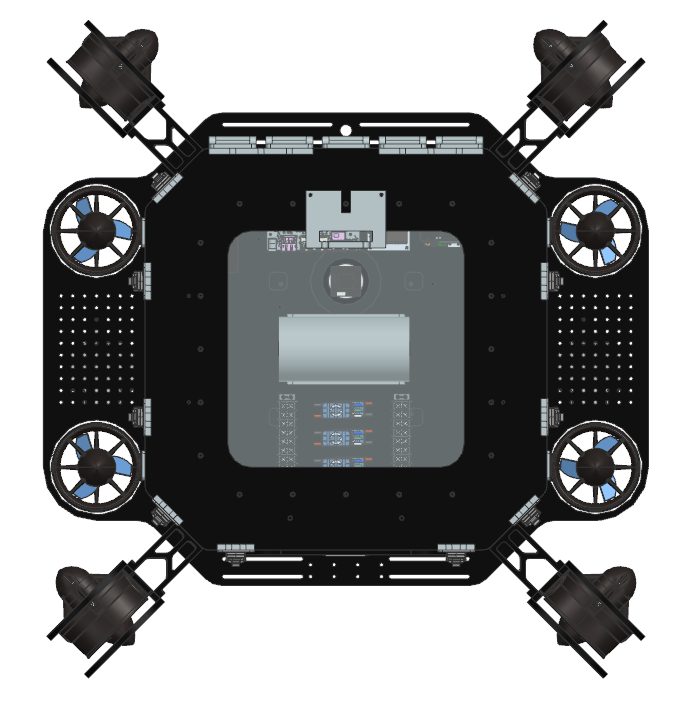
\includegraphics[scale=0.19]{images/fullSubTop2024.png}}
    \caption{CAD of top-view of Wettstein.}
    \label{fig:sub3}
\end{figure}

\subsubsection{Hull}
\label{sssec:hull}
Our hull is machined from 6061 aluminum with half inch walls to allow for long term reusability. It is a component we recovered from our previous AUV to reduce the cost of manufacturing and its modularity characteristics enable easy modifications. It has three windows, two for a front camera and bottom camera and one that provides visibility to the electrical systems for quick troubleshooting. A double o-ring face seal was used at each port to create a redundant seal that ensures a reliable leak proof sub. A lid is mounted to the hull via hinges and secured in place using latches when the sub is underwater. This hinge and latch system makes accessing electronics a quick and simple process. The submarine also contains an eight-thruster configuration, allowing it to move in all six degrees of freedom.

Besides this base hull component, our AUV was completely refurbished and redesigned for strength and modularity. With additional components this year, including a grabber and a dropper mechanism, we had to modify the frame around our hull to allow for the mounting of these components while also keeping the vehicle light enough to be at least slightly positively buoyant. We machined and installed a new bottom plate with a plethora of holes and slots to allow us to shift components and ballast weights as we test for weight distribution purposes and prevent unnecessary redesigns. This bottom plate also served the purpose of protecting the sub’s vertical thrusters from impacts. 

In addition to redesigning the AUV’s bottom plate, we also machined new mounts for its angled thrusters. These mounts contained thruster shrouds to protect the angled thrusters from wall collisions. The addition of these shrouds, as well as a new bottom plate, increased the weight of the sub. To account for this additional weight, we redesigned the lid of our hull, primarily reducing its thickness, and by extension, its weight. This redesign allowed us to discard a significant portion of buoyancy foam mounted to the top of the vehicle. 

\subsubsection{Grabber}
\label{sssec:grabber}

To pick up and move samples, we implemented a claw mechanism (Fig \ref{fig:grabber}). Our design features servo-actuated claw arms linked through a set of gears, which spin in opposite directions. When the gears spin in one direction, the claws move farther apart until a large enough gap between them opens for them to grab a sample. And when the gears spin in the other direction, the arms move closer together until they firmly clamp onto the sample. The arms were SLA 3D printed due to their complicated geometries. They are stiff enough to pick things up and hold them, while still remaining weaker than the rest of the mechanism so that they break first in case of a collision as they are much easier to make and less expensive to replace.

\begin{figure}
    \centerline{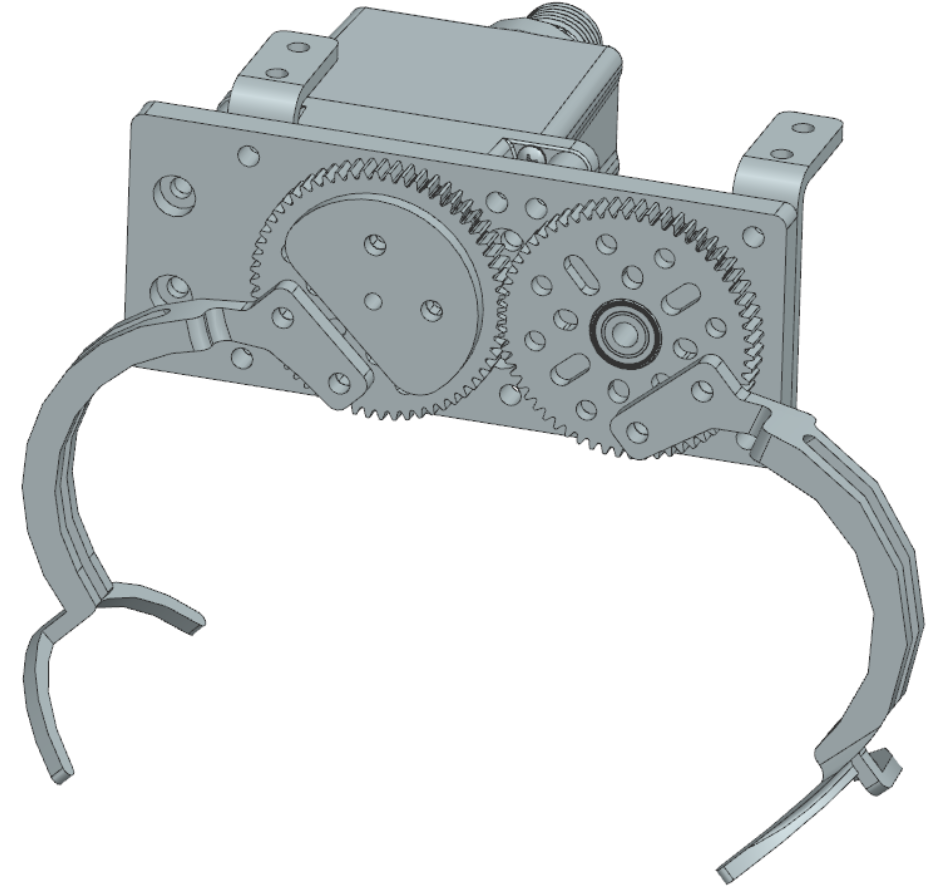
\includegraphics[scale=0.13]{images/grabberPicNew.png}}
    \caption{CAD of our grabber.}
    \label{fig:grabber}
\end{figure}

\subsubsection{Dropper}
\label{sssec:dropper}
This year, we also implemented a marker dropper subsystem (Fig \ref{fig:dropper}). Rather than employing one dropper containing two markers, we incorporated two identical droppers, with one marker in each to improve the reliability by eliminating the possibility that two markers would unintentionally be dropped simultaneously. Each dropper consists of a 3D printed tubular component in which the marker is stored. To hold the marker in place before an intended drop, a bent sheet metal arm partially blocks the bottom opening of the tube. To release the marker, a servo connected to this arm is actuated, uncovering the bottom opening of the tube and allowing the marker to fall. 3D-printing large components of the marker droppers was a quick and easy way to produce the complex shapes incorporated into the design.

\begin{figure}
    \centerline{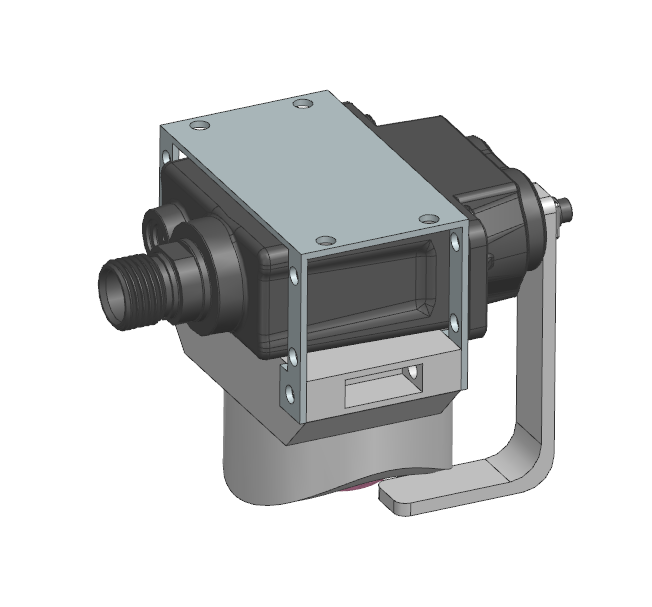
\includegraphics[scale=0.22]{images/dropperNew.png}}
    \caption{CAD of our dropper.}
    \label{fig:dropper}
\end{figure}

% \begin{figure}[h]
%     \centerline{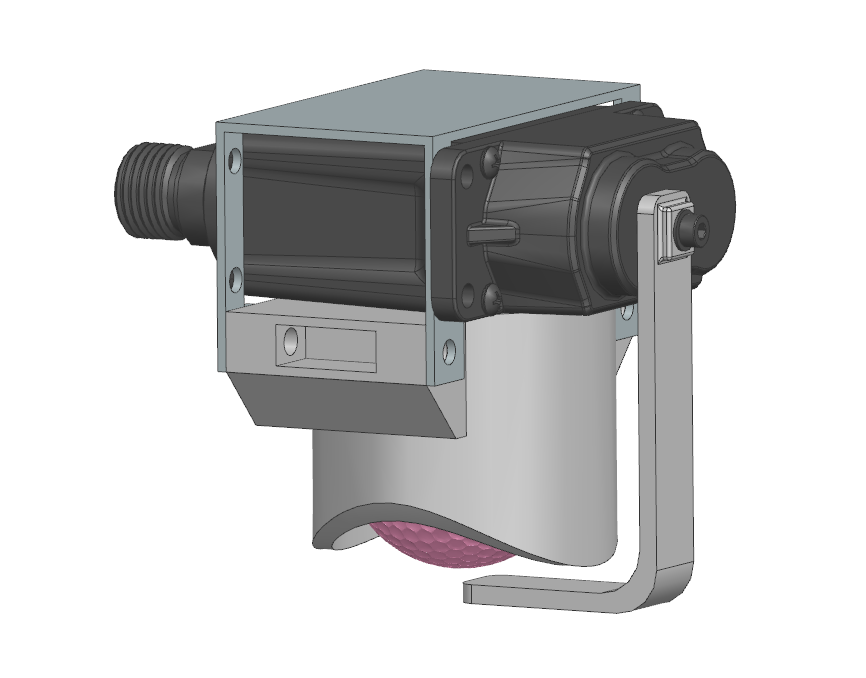
\includegraphics[scale=0.5]{images/Dropper.PNG}}
%     \caption{CAD of the dropper mechanism which mounts to the bottom plate of the hull.}
%     \label{fig:sub3}
% \end{figure}

\subsection{Electrical}
\label{ssec:electrical}


\subsubsection{Hall Effect Sensors}
\label{sssec:hall_effects}
To control the behavior of the AUV while disconnected from its tether, we used two latching hall effect sensors. These can be triggered with magnets to control the starting, stopping, and resetting of our sensors (in particular, the IMU) without needing a connection to a computer. The ability to quickly control the state of our sensors externally improves the efficiency of our testing setup time. Once a state is activated, an indicator LED is lit for visual verification. 
This year, we designed a custom PCB and 3D printed mount for our hall effect system. Previously, the hall effect sensors faced frequent disconnections due to loose wires. Additionally, the many wires needed for the hall effect system contributed to overcrowding of the electrical system. The hall effect PCB and mount remedied this issue by quartering the number of wires strengthening the connectedness of our hall effect system.

\subsubsection{Motor Control Board}
\label{sssec:motor_board}
We identified the motor control electrical subsystem as a top priority due to its critical functionality, frequency of maintenance, and large space overhead. Previously, each of our eight thrusters had 3 long wires routing across the bottom of the AUV's hull. These 24 wires would connect to eight electronic speed controllers (ESCs) and then output to eight PWM signals which are controlled by the flight controller. In practice, this setup made the subsystem difficult to organize and maintain. For instance, the process to change an ESC was lengthy and prone to breaking other components. 

As a result, we chose to encapsulate all of these wires and components into a custom printed circuit board (Fig. \ref{fig:motor_pcb}). We now have two sets of Motor-ESC boards (one on each side of the robot), where each set takes input from 4 thrusters and outputs 4 PWM signals. The ESCs mount directly to the PCB with screw-block terminals, so we can easily unscrew and swap them out. The thruster motors and PWM output connect to the PCB using Molex connectors which provide strong connections and can be disconnected easily if needed. This makes swapping out ESCs easier when necessary and frees space inside the AUV for other components.

\begin{figure}[htbp]
    \centerline{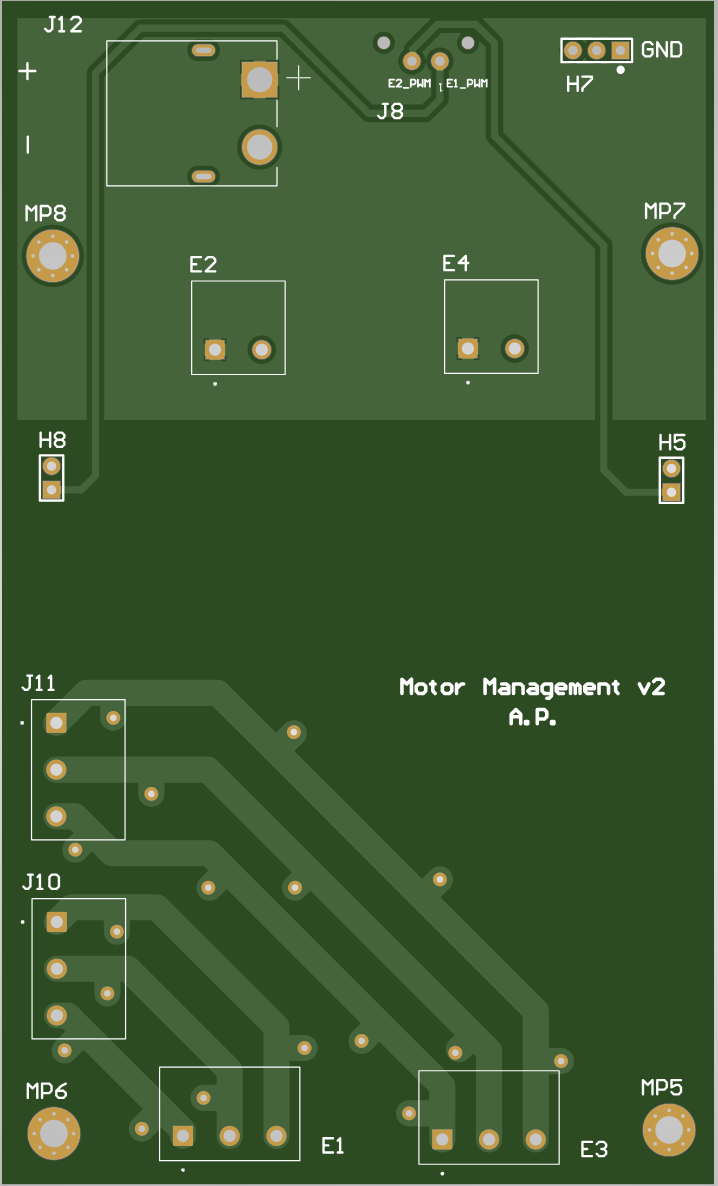
\includegraphics[scale=0.3]{images/motor_pcb.png}}
    \caption{Motor control board PCB design}
    \label{fig:motor_pcb}
\end{figure}

An important consideration was the current limit for this PCB. The first iteration of this board was operational but failed during prolonged water testing due to insufficient current rating and heat dissipation. The issue was that each ESC could theoretically draw up to 30A which meant the board’s traces had to support this requirement. Increasing the trace width to support 30A wasn’t a good use of space, so we decided to increase the copper weight of each trace, essentially making them ``taller." Additionally, we used techniques like dissipating heat with thermal vias and large power and ground planes to fully allow our motor control board to work with multiple ESCs and motors for the second iteration of the board which is currently in use.

\subsubsection{Voltage Regulation}
\label{sssec:voltage_regulation}
We continue to use our custom power distribution PCB, which utilizes an off-the-shelf Pololu 5V 15A Step Down Regulator as our DC-DC converter to supply up to 75 W to most of our electrical system components. We utilize a separate OTS DC-DC converter to supply the Jetson Xavier NX with 13V.

\begin{figure}[htbp]
    \centerline{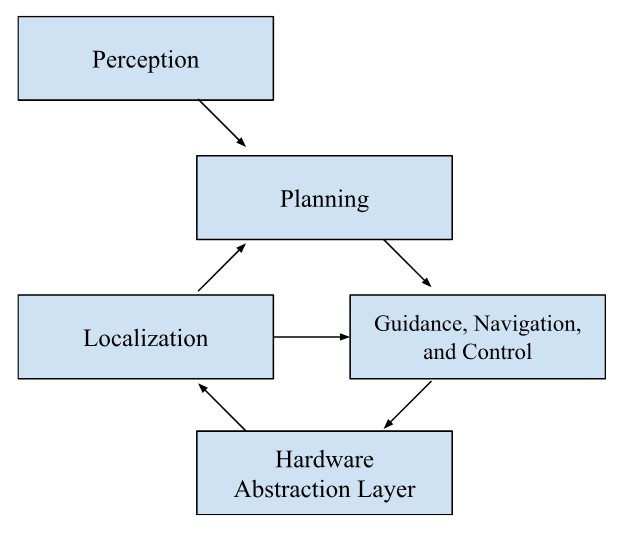
\includegraphics[scale=0.47]{images/ros_diagram.jpg}}
    \caption{High-level Software Architecture}
    \label{fig:ros}
\end{figure}
\subsection{Software}
\label{ssec:software}

Our software stack utilizes the Robot Operating System (ROS) to distribute our logic into distinct modules called nodes. These nodes are organized into packages based on their role in the AUV's operation. Fig. \ref{fig:ros} shows these packages, with arrows representing flow of information between packages. The majority of our code is written in Python, with the exception of the hardware abstraction layer, which is written in C. 

\subsubsection{Computing Architecture}
\label{sssec:comp_arch}
Our computing architecture features a distributed layout to enable high flexibility. Most of our computing is carried out on our Jetson Xavier NX. This is the most powerful computer in the system, so it is responsible for running our computer vision and machine learning algorithms, as well as our high level planning, localization, and control modules. Our motor control is handled by a PX4 PixHawk flight controller, which requires a Raspberry Pi 3B+ to interface with. We designed our system so that the Raspberry Pi is solely responsible for interfacing with the flight controller; this allows the rest of our code to run on the Jetson, utilizing its superior capabilities. For interfacing with our low-power devices – namely our depth sensor, hall effect sensors, and indicator lights – we use an Arduino, which the Jetson communicates with via \verb|rosserial|.

\subsubsection{Orientation Sensing}
\label{sssec:orientation_sensing}
To sense our orientation, we use the flight controller’s internal IMU (inertial measurement unit). Last year, we observed that sometimes our orientation readings would drift significantly. This year, we performed extensive diagnostics on this problem, and found that this was caused by the flight controller attempting to fuse magnetometer readings with the IMU. Due to a large amount of magnetic interference in the system, these readings were drifting. We resolved this by disabling the magnetometer, resulting in  more consistent orientation measurements.

\subsubsection{Computer Vision}
\label{sssec:cv}
In order to detect the pathmarker, buoy, and bins, we utilize classical computer vision (CV) techniques with the OpenCV library. These objects are single-colored with fewer features, making them highly noticeable with HSV thresholding. The HSV (Hue, Saturation, Value) color model simplifies the process of detecting these objects, as it aligns more closely with human perception of color and allows for more intuitive color-based segmentation \cite{b2}. Additionally, CV techniques are computationally cheaper compared to ML models, making them more suitable for real-time applications on our autonomous vehicle.

Our HSV filter pipeline has been streamlined to handle multiple tasks, including path marker, buoy, and bin detection. The approach involves several key steps to enhance and process the underwater images. First, we adjust the white balance of the image to counteract the color distortion caused by underwater conditions. This process shifts and scales the color channels to balance the overall image color, making the objects more distinguishable. Following this, we perform histogram equalization on the RGB channels of the image to enhance the global contrast, ensuring that the details of the objects stand out more prominently (Fig. \ref{fig:enhanced_compare}). The enhanced image is then converted from the RGB color space to the HSV color space. To reduce noise and smooth the image, we apply median and Gaussian filters. Next, we apply color thresholding to the HSV image to create a binary mask that isolates the object’s colors, in which the objects are highlighted against the background. The binary mask is further refined using morphological operations such as erosion and dilation to mitigate noise and fill gaps.


\begin{figure}[htbp]
    \centerline{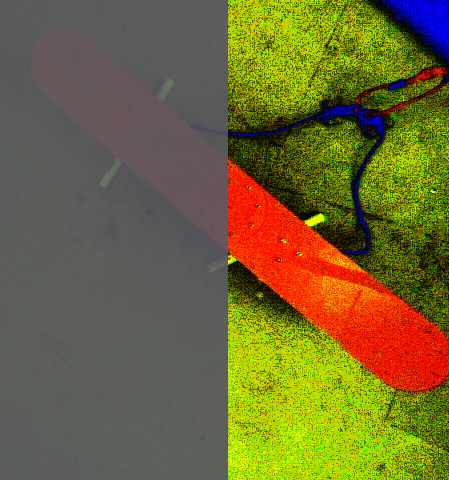
\includegraphics[scale=0.32]{images/pathmarker_compare.png}}
    \caption{Example of a pathmarker image before (left) and after (right) image enhancement.}
    \label{fig:enhanced_compare}
\end{figure}


Using the binary mask, we detect contours in the image, representing the boundaries of the objects. We analyze these contours by their size and features uniqueness to identify the desired objects. If a valid contour is found, we then process them based on the specific tasks: either path marker, buoy, or bin. For the path marker, we use the minimum area rectangle method (bounding box) to approximate the path marker's boundary. We then identify the corners of this rectangle and calculate the center points of the edges. The centers of the edges and the center of the rectangle are calculated, and we use these points to determine the yaw angle of the path marker relative to the camera's heading. By drawing lines between the corners and calculating the angles, we can determine the orientation of the path marker. This provided a significant improvement over our pathmarker detection from last year, which naively searched for lines without considering the shape of the object. For buoy detection, we employ a similar approach but focus on circular objects. The algorithm calculates the center and radius of the detected buoy to determine its position and size. For bin detection, the process is analogous to path marker detection; Fig. \ref{fig:bin_features} shows an example of detecting the key features on the object. See Appendix A for full examples of this pipeline operating on each object type.

\begin{figure}[htbp]
    \centerline{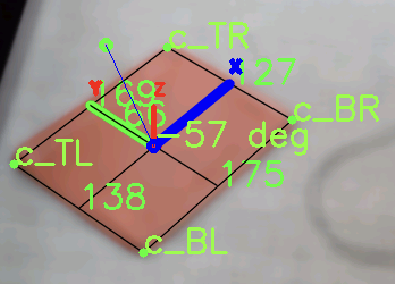
\includegraphics[scale=0.55]{images/bin_features.png}}
    \caption{Example of detecting key features on a bin-shaped object.}
    \label{fig:bin_features}
\end{figure}

One notable challenge we faced was the effects of our camera's automatic white balance adjustments. Automatic white balance adjustments can introduce variability in the color representation of objects, affecting the accuracy of HSV filtering. This variability can lead to inconsistent detection results, as the colors of the objects may appear differently under varying lighting conditions. To mitigate this issue, we prefer manual white balance settings to maintain consistent color representation and enhance the reliability of our CV pipeline.

% Redundant sentence methinks:
% By controlling the white balance manually, we ensure that the color characteristics of the objects remain stable, allowing the HSV filter to perform accurately and consistently.

\subsubsection{Machine Learning}
\label{sssec:ml_flow}
To detect the images on the gate, we continue to use the machine learning pipeline that we developed last year. We use the YOLOv5 neural network \cite{b3} for object detection, which we fine-tuned to detect gate images. Our model runs within the PyTorch framework, an open source machine learning framework that is an industry standard for this type of work \cite{b4}. 

Last year, we streamlined our process of labeling data and training models by developing a series of scripts to automate the setup of training on the Great Lakes Computing Cluster and removing the need to generate the image labels for each training run. We created a data pre-processing script that ensures all of the images were of the correct resolution, file type, and naming convention. We would then import the images to LabelBox and draw bounding boxes. A second script then generates the label files and splits them into the required train and test designations. To understand how well newly trained models perform on a test set, we utilized a model evaluation script, provided by the Ultralytics YOLO package. These evaluation metrics allow us to easily compare the performance of two models. We found at last year’s competition that this allowed us to efficiently train our model using only data we collected at the venue. Thus, we continue to leverage this pipeline, and we plan to train the model to detect the gate using images we will collect at competition.

\subsubsection{Task Planner}
\label{sssec:task_planner}
The task planner is code for coordinating system components to complete tasks during a run. Last year, we rewrote our planning framework to allow rapid changes to the task planning logic while at competition. Namely, this system allows us to easily modify the transitions between different behavior states without modifying the states itself.

At competition last year, we ran into several issues in our task planning code that could have been prevented by increased static code analysis, including mistyped variable names and unexpected type errors. We were unable to run static analysis on our code because of the highly dynamic code in the state machine. This year we enhanced the framework by making the state machine implementation type safe and requiring code written with the state machine to be type safe. We check the type safety with \verb|mypy|, a Python linter and type checker. The additional type safety also lets our development environment provide much more relevant and useful auto-complete suggestions, increasing developer productivity.

An additional benefit of the state machine refactors is that we were able to add the ability to automatically create a visualization of the state machine. These visualizations convert the state machine transition maps into a flow visualization graph, which allows us to visually verify the logic flow in the code is equivalent to the logic flow we intended. Appendix B includes an example of such a graph generated from our complete state machine.

% \subsubsection{Path Marker Detection}
% \label{sssec:path_marker}

% \subsubsection{Glyph and Object Detection}
% \label{sssec:glyph_object_detection}

% \subsubsection{Machine Learning Process}
% \label{sssec:ml_flow}

\section{Testing and Experimental Results}
\label{sec:testing}

\subsection{Teleoperation Framework}
\label{ssec:teleop}
A key takeaway from competing in-person last year was the need for an efficient water testing infrastructure. Due to the interdependence of our subsystems, it is challenging to test individual components of our system while the AUV is operating autonomously; it is often difficult to diagnose the source of errors when the entire system is running.

Last year, we developed a robust teleoperation (teleop) framework that allows a human driver to manually control various aspects of the AUV while other subsystems run autonomously, enabling us to quickly and efficiently execute unit tests and debug components in isolation. Our framework makes significant improvements compared to the default manual control system provided by ArduSub on our Pixhawk flight controller, including faster switching between autonomous / teleoperated modes, ability to alter the control mode of each degree of freedom separately, and more reliable emergency stopping. We found that this greatly expedited our testing process during last year’s competition, and thus we continued to develop and utilize this framework.

\subsection{In-Water Testing}
\label{ssec:in_water_testing}
From past competitions we have learned that in-water testing is invaluable and allows for both the software and hardware teams to validate their designs. It also provides a great opportunity for training new members and boosts morale. For these reasons our team has attempted to utilize our Universities resources to perform as many water tests as possible.

We used a water tank in the Ford Motor Company Robotics Building (FMCRB) at the University of Michigan to perform unit tests and sensor, motor, and camera calibrations. We performed control parameter tuning and movement testing at the U-M Marine Hydrodynamics Laboratory (MHL), along with larger-scale tests that involved competition elements.

Before each in-water testing session, we wrote a test plan which describes what specific tests are to be carried out and explains the high-level purpose of each test. We recorded the procedure for each task and the expected results, along with some notes on potential problems or bugs. This allowed us to streamline testing once we arrived on-site and allowed us to create a log of tests we’ve previously performed and issues we’ve previously encountered. 

% See Appendix C for a sample test plan. 

Throughout the fall, we performed significant enhancements to the mechanical components and electronic system. In order to validate the various changes we made, we performed several smaller unit-tests using the water tank at the FMCRB. Once the system was stable during the spring, we were able to perform many larger in-water tests at the MHL. These tests included tuning and evaluating the computer vision pipeline, profiling our movement, and attempting full competition tasks. Also, when at the MHL, we would collect image data of the various tasks so that we could test and tune our computer vision algorithms offline. Over the course of the spring and the summer, we typically performed between two and four water tests per month. 

As we incrementally added new components to the hull of the AUV, we assessed how they affected the modified weight distribution, movement, and PID tuning of the AUV using several in-water unit tests. These included driving in a square and driving forward, both at a set depth. The physical testing also proved to be beneficial for incremental changes in our submarine to improve the efficiency and reusability. These changes were primarily driven by our number of collisions while testing, the specific orientation and movement that each collision had, as well as how well our submarine fared with our wet mate connector. This led to a number of changes that overall hardened our sub so that it could take hits without breaking all the time -- primarily by adding metal cases to outer components, 3D printing other components so that they break instead of more crucial components, and moving the parts around with a more modular design.


\subsection{Off-Board Testing}
\label{ssec:off_board_testing}
In order to write, execute, and test our software off of the AUV, we developed a Docker image that emulates our main computer. This workflow allows anyone on our team to quickly set up our development environment on their computer. In general, we tested the logic of our software off-board of the AUV and reserved in-water testing for collecting data to improve our vision system or test the physical results of the algorithms once they had been tested in simulation. This prevented valuable in-water testing time from being consumed with simple software errors.

We also developed a Unity simulation that communicates with our software emulation in Docker. We wrote Unity C\# software to simulate the movement, sensor data, and vision data of the AUV with random statistical noise. The simulation also enables us to evaluate our software's behavioral logic within a to-scale Transdec scene created by Team Inspiration \cite{b5} (see Fig. \ref{fig:unity}).

To visualize the output of our software both in Docker and on the real AUV, we created visualizations using RQt, a ROS dashboard library. We leveraged RQt to graph data and dynamically tune control parameters, allowing for easy incremental testing.

\begin{figure}[htbp]
    \centerline{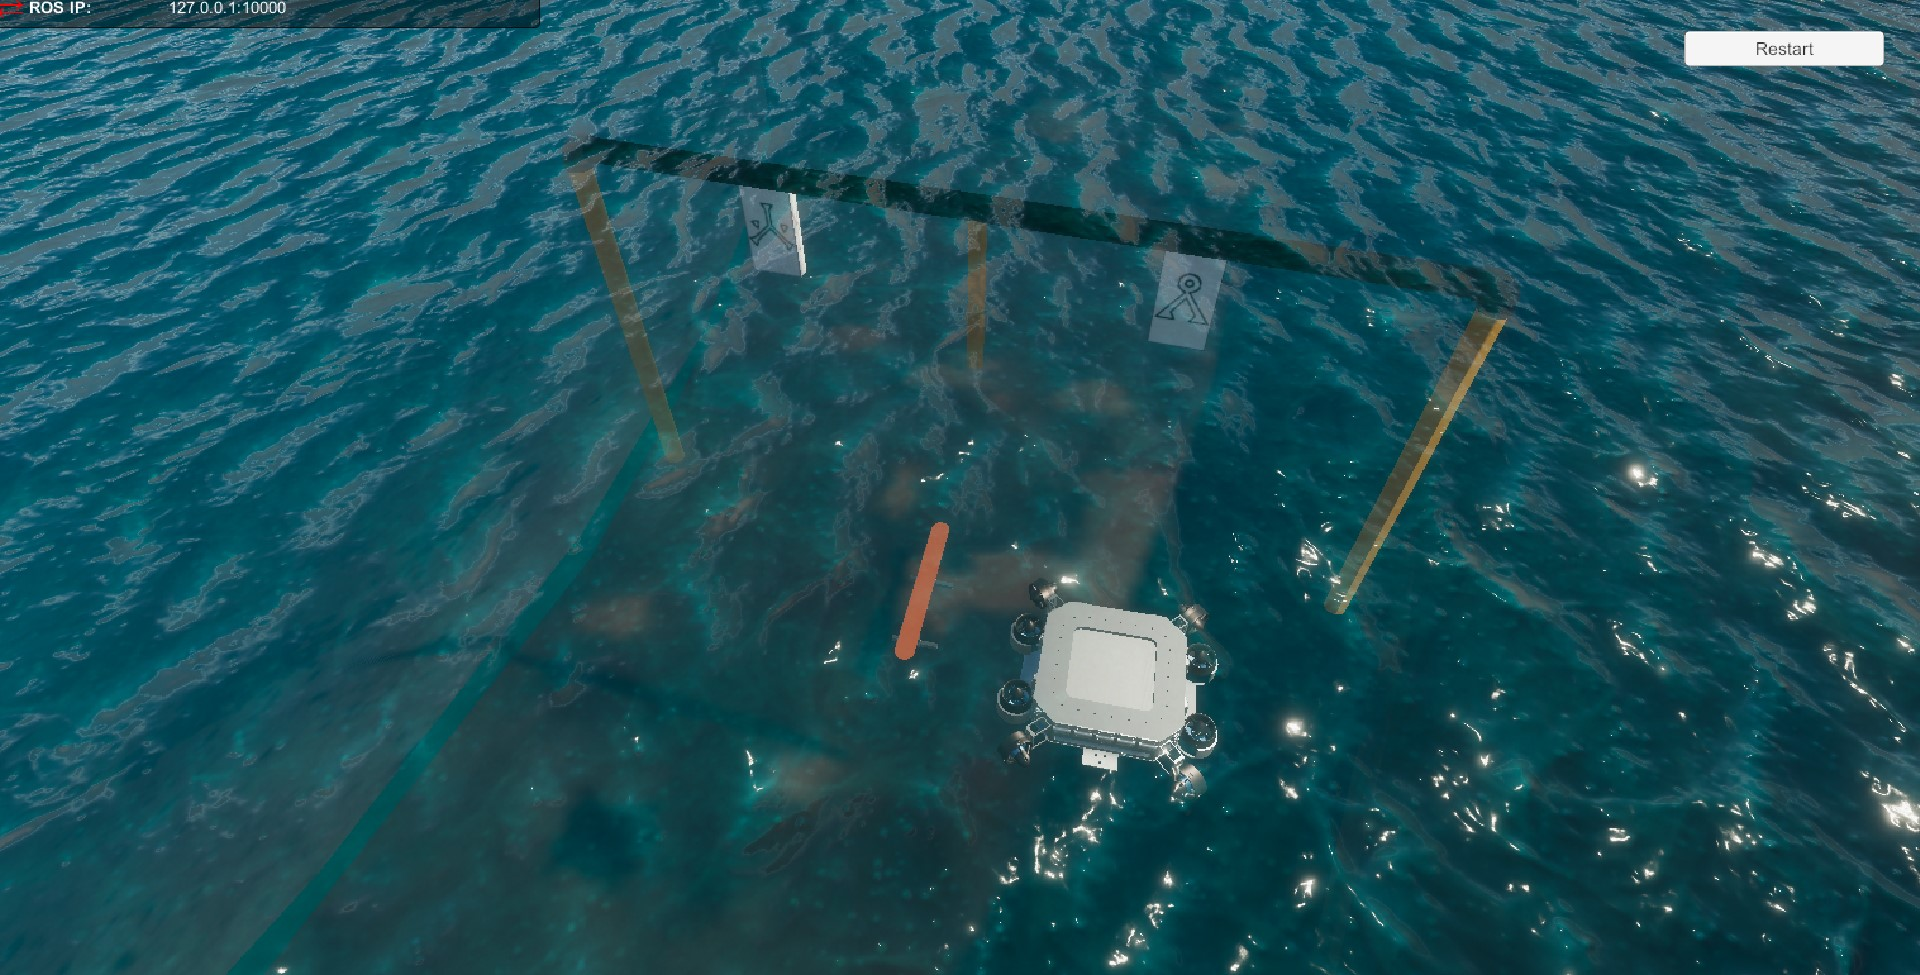
\includegraphics[scale=0.16]{images/unity_new.jpg}}
    \caption{Testing the gate task logic using Docker and Unity.}
    \label{fig:unity}
\end{figure}

\section*{Acknowledgements}

The Michigan Robotic Submarine team would like to thank our 2024 sponsors for their monetary support: Ford Motor Company, University of Michigan Central Student Government, the University of Michigan College of Engineering along with the departments: Robotics, Computer Science and Engineering, Electrical and Computer Engineering, and Mechanical Engineering. We'd also like to thank the individuals who donated to our team during the University of Michigan's Giving Blue Day fundraiser. 

In addition, we would like to thank our advisor Dr. Katie Skinner for continuously supporting our team by advising us and overseeing the Multidisciplinary Design Program which allows members to earn class credit for their contributions to our team.

We are greatly appreciative of the Marine Hydrodynamics Lab staff, especially Jason Bundoff and Nicole Cheesman, for graciously providing the team with an in-water testing location. 

We also would like to thank the Wilson Student Team Project Center facilities and Ford Motor Company Robotics Building staff, especially Alyssa Emigh and Chris Gordan, for hosting our team workspace, providing tools and resources, and supporting our endeavors. 

We are also thankful of Mariah Moss and Katelyn Poore from the Office of Student Affairs at the University of Michigan College of Engineering for their guidance in developing our team and assistance purchasing the materials that make our work possible. 

Lastly, we would like to thank the RoboNation team for organizing the RoboSub competition. We are also thankful for the hydrophone and image data provided through the RoboNation data sharing program.

\begin{thebibliography}{00}
% \bibitem{b2} A. Zelenak, ``A PID controller for ROS". bitbucket.org. https://bitbucket.org/AndyZe/pid/src/master/ (accessed June 11, 2022)
\bibitem{b2} N. Fragoulis and D. Kastaniotis, “Why Embedded Software
Development Still Matters: Optimizing a Computer Vision Application
on the ARM Cortex A8.” 2013, publisher: Irida Labs. [Online].
Available: http://rgdoi.net/10.13140/2.1.2670.6240
\bibitem{b3} G. Jocher, ``ultralytics/yolov5: v6.1 - TensorRT, TensorFlow Edge TPU and OpenVINO Export and Inference”. Zenodo, Feb. 22, 2022. doi: 10.5281/zenodo.6222936.
\bibitem{b4}{P. Adam et al., ``PyTorch: An Imperative Style, High-Performance Deep Learning Library", in Advances in Neural Information Processing Systems 32, Curran Associates, Inc., 2019, pp. 8024–8035.}
\bibitem{b5} Inspiration Robotics, ``RoboSub-Simulation". Github.com. https://github.com/InspirationRobotics/RoboSub-Simulation (accessed June 11, 2022)

\end{thebibliography}

\clearpage
\appendices

\raggedbottom

\pagebreak
\section{Computer Vision Pipeline Results}

% \vspace{0.5cm}
% 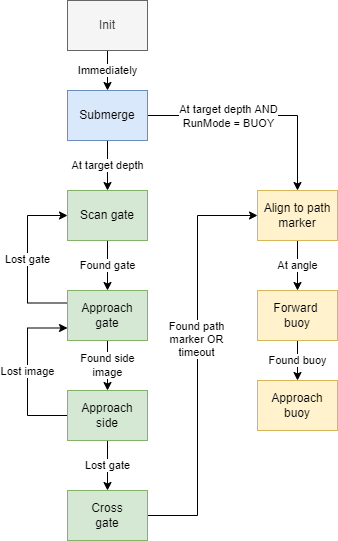
\includegraphics[scale=0.6]{images/task_state_machine.png}

\vspace{0.5cm}
\includegraphics[scale=0.42]{images/cv_pipeline.drawio.png}
\newpage
\clearpage


\section{State Machine Diagram}
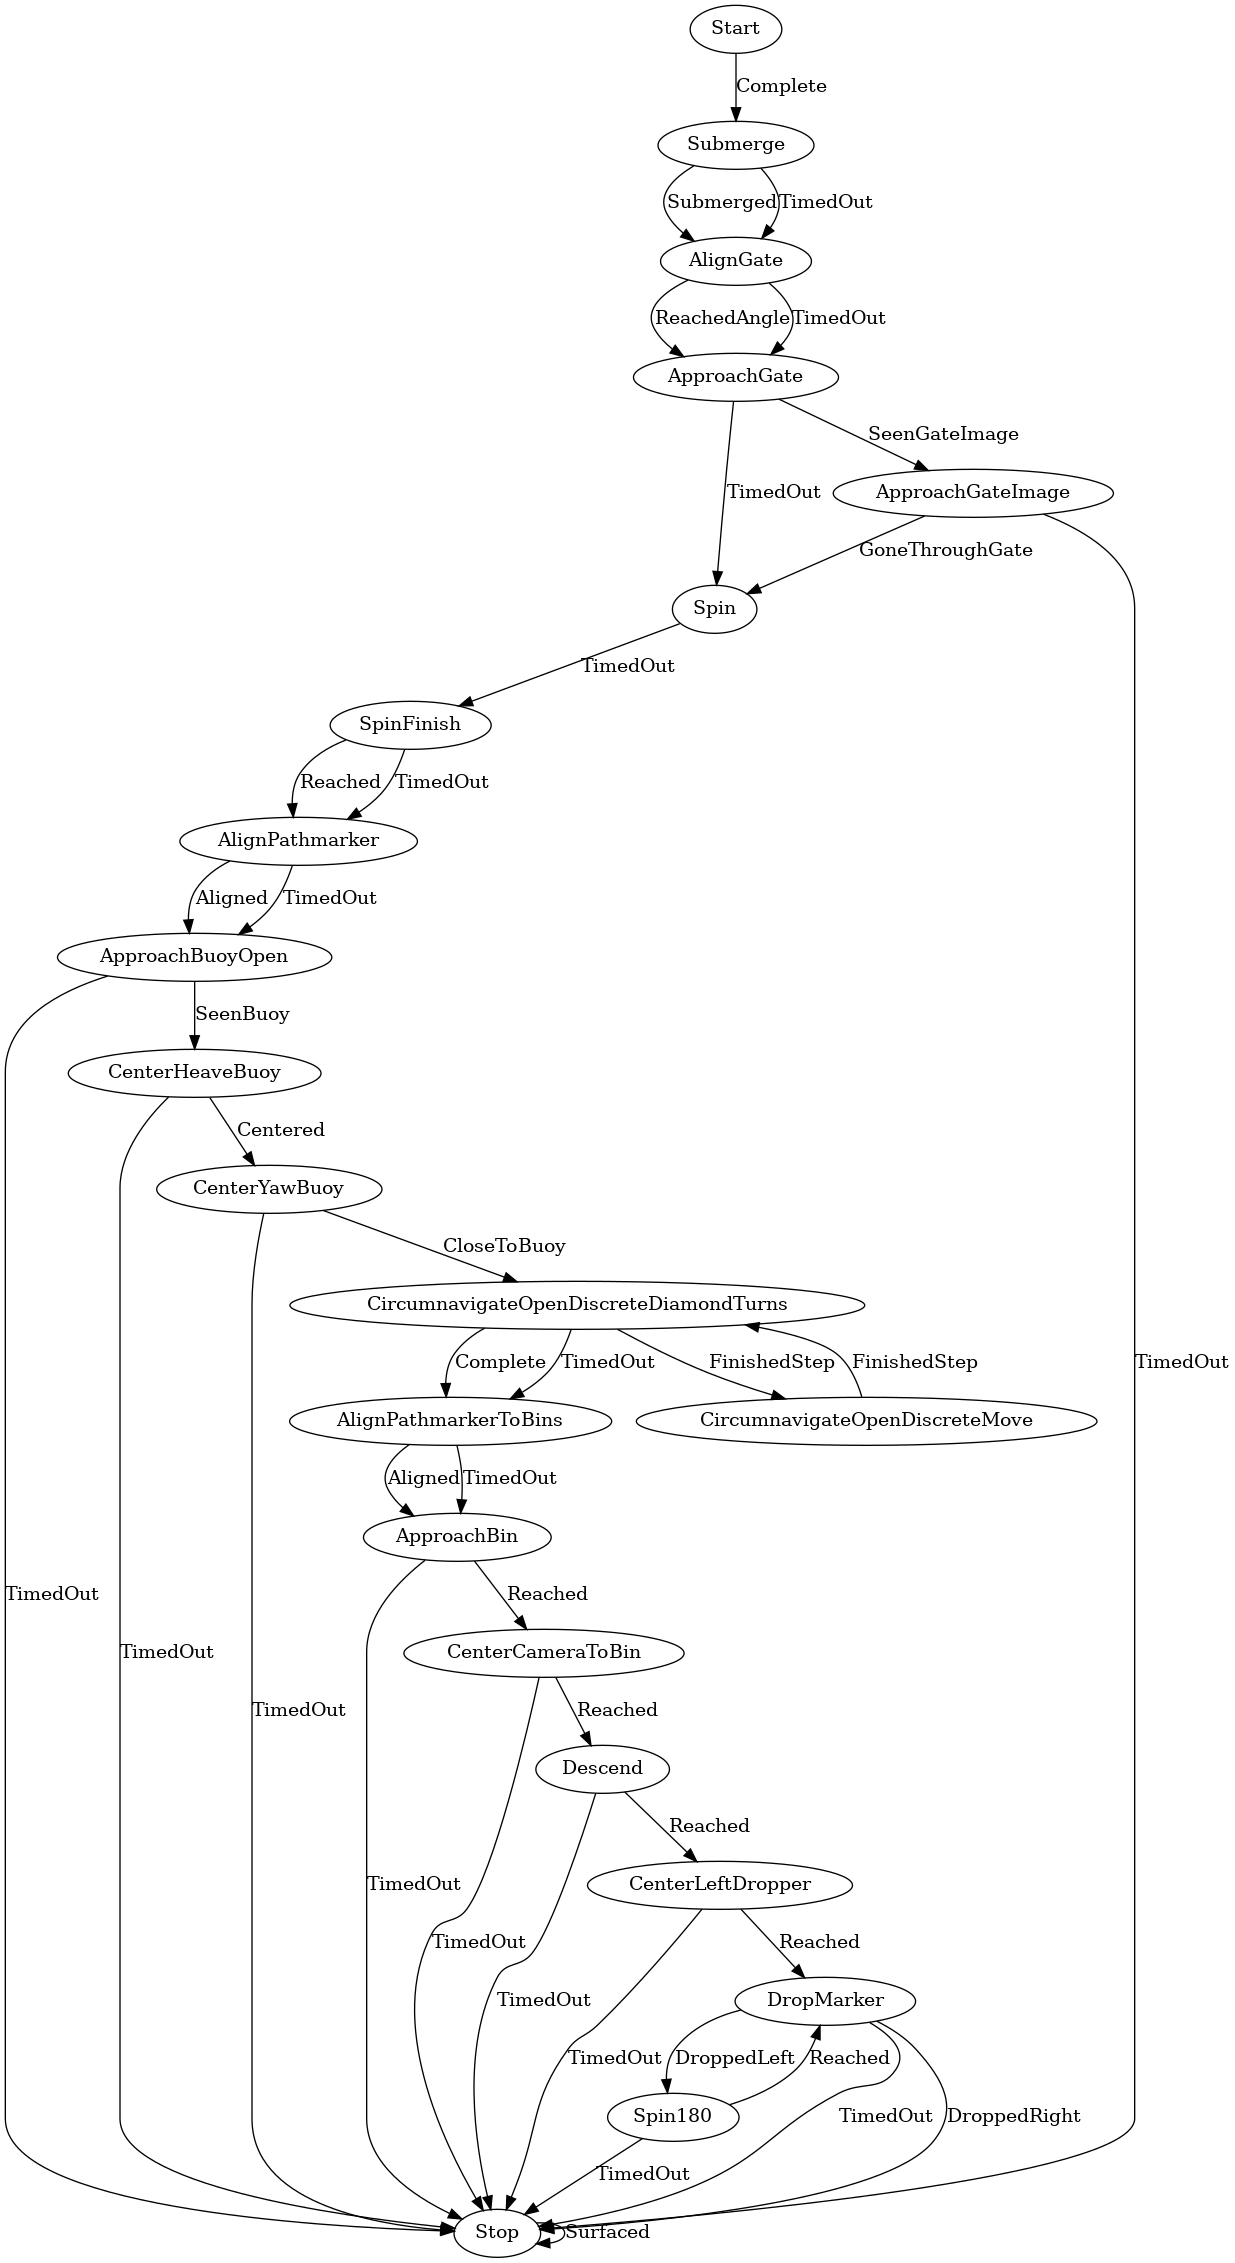
\includegraphics[scale=0.27]{images/machine2.png}
\newpage

\clearpage
\section{Component Specifications}

% \begin{center}
\begin{table}[htbp]
\begin{tabularx}{\textwidth}{|X|X|X|X|X|X|}
    \hline
        Component & Vendor & Model/Type & Specs & Cost (if new) & Year of Purchase \\ \hline
        ASV Hull Form/Platform  & American Tooling \& Prototype & Custom & 6061 Aluminum & \$3250.00 & 2022 \\ \hline
        Waterproof Connectors & Blue Robotics & WetLink Penetrators & WLP-M10-6.5MM-HC & \$120.00 & 2024 \\ \hline
        Propulsion  & Blue Robotics & T200 w/ Propellor & 7-20V & \$1,074.00  & 2020\\ \hline
        Power System & N/A & Custom & N/A & N/A & N/A \\ \hline
        Motor Controls  & Blue Robotics & Basic ESC & 7-26V & \$172.00  & 2023 \\ \hline
        CPU & Nvidia & Jetson Xavier NX & 6-core Nvidia Carmel ARM v8.2 @ 1.9 GHz, 16 Gb RAM & \$400.00  & 2022 \\ \hline
        Compass  & PixHawk & PX4 & Accel/Gyro: ICM-20689 with Magnetometer & \$189.99  & 2022 \\ \hline
        Inertial Measurement Unit (IMU)  & PixHawk & PX4 & MPU6000 9-axis & 189.99 & 2022 \\ \hline
        Doppler Velocity Log (DVL) & N/A & N/A & N/A & N/A & N/A \\ \hline
        Camera(s) & Stereolabs, Blue Robotics & ZED2, Low-light HD USB Camera & stereo vision, pathmarker detection & \$449.00, \$99.00  & 2020, 2021 \\ \hline
        Hydrophones & N/A & N/A & N/A & N/A & N/A \\ \hline
        Localization and Mapping  & N/A & Custom & N/A & N/A & N/A \\ \hline
        Vision  & N/A & YOLOv5, PyTorch, OpenCV & train convolutional neural network and perform classical computer vision & N/A & 2023 \\ \hline
        Autonomy  & N/A & Custom & N/A & N/A & N/A \\ \hline
        Open source software & N/A & Andy Ze ROS PID & PID Control & N/A & N/A \\ \hline
    \end{tabularx}
\label{tab1e}
\end{table}



\end{document}
